\item \textbf{{[}NYJC/PRELIM/9597/2019/P1/Q3{]} }

Create a binary tree Abstract Data Type (ADT) with commands to create
a new tree, insert data items to the tree and print the tree. 

The sequence of commands 
\noindent \begin{center}
\begin{tabular}{l}
Create a new tree\tabularnewline
Add to tree (15) \tabularnewline
Add to tree (10) \tabularnewline
Add to tree (20) \tabularnewline
Add to tree (8) \tabularnewline
Add to tree (12) \tabularnewline
Add to tree (18) \tabularnewline
Add to tree (25)\tabularnewline
\end{tabular}
\par\end{center}

would create the following binary tree: 
\begin{center}
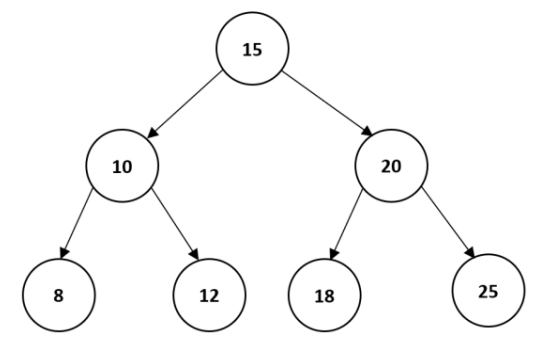
\includegraphics[width=0.25\paperwidth]{C:/Users/Admin/Desktop/Github/question_bank/LyX/static/img/9597-NYJC-2019-P1-Q3-1}
\par\end{center}

The program to implement this ADT will use the classes Tree and Node
designed as follows: 
\begin{center}
\begin{tabular}{|l|}
\hline 
\texttt{ToDo}\tabularnewline
\hline 
\texttt{root : Node}\tabularnewline
\hline 
\texttt{constructor()}\tabularnewline
\texttt{add(newItem)}\tabularnewline
\texttt{printTreeInOrder()}\tabularnewline
\hline 
\end{tabular}%
\begin{tabular}{|l|}
\hline 
\texttt{Node}\tabularnewline
\hline 
\texttt{key : INTEGER}\tabularnewline
\texttt{left : Node}\tabularnewline
\texttt{right : Node}\tabularnewline
\hline 
\texttt{constructor()}\tabularnewline
\texttt{insert(key : INTEGER)}\tabularnewline
\hline 
\end{tabular}
\par\end{center}

\subsection*{Task 3.1 }

Write program code to define the classes \texttt{Tree} and \texttt{Node}.

\subsection*{Evidence 8: }

Your program code. \hfill{}{[}16{]}

\subsection*{Task 3.2 }
\begin{itemize}
\item Write program code for a procedure \texttt{CreateTreefromArray} that
accepts an array of unsorted unique integers passed in via a parameter. 
\item The procedure will read each integer in the array and construct a
binary tree using your classes \texttt{Tree} and \texttt{Node}. 
\item Call \texttt{printTreeInOrder} to display the output (numbers shown
will always be sorted). 
\item Test your program by copying the input data found in \texttt{BST.txt}
into your code. 
\end{itemize}

\subsection*{Evidence 9: }

Your \texttt{CreateTreefromArray} program code. \hfill{}{[}4{]}

\subsection*{Evidence 10: }

A screenshot of the output. \hfill{}{[}2{]}

\subsection*{Task 3.3}

A binary tree created from keys that are in ascending order will result
in an unbalanced binary tree.

For instance, the sequence of commands
\noindent \begin{center}
\begin{tabular}{l}
Create a new tree \tabularnewline
Add to tree (8) \tabularnewline
Add to tree (10) \tabularnewline
Add to tree (12) \tabularnewline
Add to tree (15)\tabularnewline
Add to tree (18) \tabularnewline
Add to tree (20)\tabularnewline
Add to tree (25)\tabularnewline
\end{tabular}
\par\end{center}

will result in a tree that looks as follows: 
\begin{center}
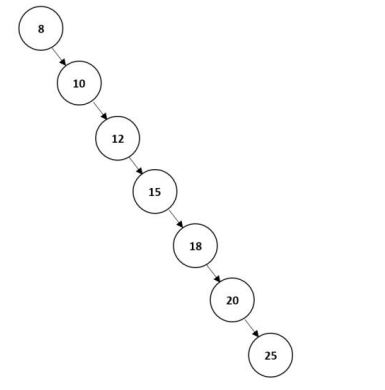
\includegraphics[width=0.25\paperwidth]{C:/Users/Admin/Desktop/Github/question_bank/LyX/static/img/9597-NYJC-2019-P1-Q3-2}
\par\end{center}

Amend procedure \texttt{CreateTreefromArray} so that the created tree
from any input array of integers will be balanced where the number
of items on the left and right subtree will roughly be divided equally
(Hint: input array must first be sorted).

\subsection*{Evidence 11: }

Your amended program code. \hfill{}{[}6{]}

\subsection*{Task 3.4 }

Create a function \texttt{FindKthSmallest} that returns the $k$th
smallest element in your binary tree. If $k=5$ the $k$th smallest
element will be 18. Your function should not need to use extra space
(e.g. creating a new array) to solve the problem other than using
a temp variable(s). 

\subsection*{Evidence 12: }

Your program code for \texttt{FindKthSmallest}. \hfill{}{[}4{]}

\subsection*{Evidence 13:}

Produce a screenshot showing the retrieval of the 5th smallest element
from the tree created earlier. \hfill{}{[}2{]}